\documentclass[11pt]{article}

\usepackage[margin=1.1in]{geometry}
\usepackage{amsmath}
\usepackage{amssymb}
\usepackage{booktabs}
\usepackage{graphicx}
\usepackage[hidelinks]{hyperref}

% One symbol per object, used consistently.
\newcommand{\bone}{b_1}            % Eulerian linear bias
\newcommand{\btwo}{b_2}            % Eulerian quadratic bias (CCL convention)
\newcommand{\bs}{b_{s^2}}          % Eulerian tidal bias (CCL convention)
\newcommand{\bthree}{b_{3\mathrm{nl}}} % Eulerian third-order bias (CCL convention)
\newcommand{\boneL}{b_1^{\mathrm{L}}}
\newcommand{\btwoL}{b_2^{\mathrm{L}}}
\newcommand{\bsL}{b_s^{\mathrm{L}}}
\newcommand{\bthreeL}{b_3^{\mathrm{L}}}
\newcommand{\plin}{P_{\mathrm{lin}}}
\newcommand{\pnl}{P_{\mathrm{mm}}}
\newcommand{\kmax}{k_{\mathrm{max}}}
\newcommand{\hMpc}{\,h\,\mathrm{Mpc}^{-1}}
\newcommand{\Mpch}{\,h^{-1}\mathrm{Mpc}}
\newcommand{\aunit}{\,h^{-2}\mathrm{Mpc}^2}
\newcommand{\SNz}{\mathrm{SN}_0}
\newcommand{\SNt}{\mathrm{SN}_2}

\emergencystretch=2em

% Floats sit near their first reference instead of drifting to
% figure-only pages.
\renewcommand{\topfraction}{0.9}
\renewcommand{\bottomfraction}{0.8}
\renewcommand{\textfraction}{0.07}
\renewcommand{\floatpagefraction}{0.85}
\setcounter{topnumber}{3}
\setcounter{totalnumber}{4}

\title{Higher-order galaxy bias for DESI thin-bin angular clustering\\
\large The one-loop bias model of the lssty1xdesi project}
\date{November 2026}
\author{}

\begin{document}
\maketitle

\begin{abstract}
\noindent
The lssty1xdesi forecast combines LSST Y1 3x2pt with DESI angular
galaxy clustering $C_\ell^{gg}$ in thin redshift bins, computed without
the Limber approximation.  This note describes the one-loop galaxy bias
model of its DESI likelihood and the physics behind each choice.  The
model is one likelihood option with every term per bin: the real-space
one-loop Eulerian bias expansion on a per-bin linear bias, with the
quadratic and tidal biases tied to calibrated relations plus group
offsets, a $k^2$ counterterm, the redshift-space counterterm $\alpha_2$
in the DESI DR1 convention, and two stochastic terms, a white noise
$\SNz$ and a line-of-sight term $\SNt k^2\mu^2$.  Models A and B are
two parameter files of this option: model A, built for
$\kmax = 0.075\hMpc$, fixes $\alpha_2 = 0$; model B frees it and
doubles the offset widths; the paper model is model B + tilts with
$\alpha_2 = 0$ in every bin and every $\sigma_v$ prior width multiplied
by six.  Every term projects exactly: $\alpha_2$
through the Kaiser transfers, $\SNt$ through the radial derivatives of
the bin kernels.  That derivative structure anticorrelates the
projected $\SNt$ of neighboring thin bins, a pattern no white noise
reproduces; without $\SNt$, model A fails on the thin layouts at its
own cut.  The draft paper's bias table holds the DESI DR1 sampling
combinations of Lagrangian biases, not Eulerian biases, so the model
takes its fiducials from the calibrations.  The loop terms change the
galaxy power by up to $7\%$ at model A's per-bin cut and up to $15\%$
at the shipped mask.
\end{abstract}

\tableofcontents

\section{Scope and conventions}
\label{sec:scope}

The lssty1xdesi project forecasts DESI spectroscopic galaxy clustering
as angular power spectra $C_\ell^{gg}$ in thin redshift bins, combined
with LSST Y1 3x2pt.  The DESI spectra are computed on four bin
layouts: 76 bins of equal comoving width
($\Delta d_{\rm com} = 62$\,Mpc), and bins of fixed redshift width
$\Delta z = 0.02$, $0.05$ and $0.2$.  The bins fall into six tracer
groups: BGS, LRG1, LRG2, LRG3, ELG1 and ELG2.  A bin of comoving width
$\Delta\chi$ resolves radial Fourier modes up to
$k_\parallel \simeq \pi/\Delta\chi$, about $0.075\hMpc$ for the
$62$\,Mpc bins, so the angular analysis recovers most of the
three-dimensional information at that scale \cite{Asorey2012}.

With linear bias the likelihood models the galaxy power as
$P_{gg} = \bone^2\pnl$, with $\pnl$ the halofit matter power spectrum,
and a linear-bias fit holds only to $\kmax = 0.05\hMpc$ on this data
vector (\texttt{notes/linear\_bias\_kmax}).  This note describes the
one-loop model that replaces it: the fiducial parameter values behind
the note (Section~\ref{sec:fiducial}), the physics the model rests on
(Sections~\ref{sec:oneloop}--\ref{sec:verdict}), the size of each term
(Section~\ref{sec:sizes}), the model, its two parameter files, models
A and B, and the paper model (Section~\ref{sec:model}), the exact
projection of each term to thin-bin spectra
(Section~\ref{sec:projection}), and the checks
(Section~\ref{sec:validation}).  The forecasts made with it are in
\texttt{notes/correlated\_bias\_prior\_v2}, the correlated-prior note:
the linear-bias priors and their accuracy test, model B against
$\kmax$, and where model B breaks.

\paragraph{Conventions.}
$\ell$ is the multipole; $k$ is the comoving wavenumber, in $h$/Mpc
unless a unit is written; $z$ is redshift and $\bar{z}_i$ the mean redshift of bin $i$; $\mu$ is
the cosine between the wavevector and the line of sight; $D(z)$ is the
linear growth factor, $D(0) = 1$, and $f = d\ln D/d\ln a$ the growth
rate, with $a$ the scale factor; $\sigma_8(z)$ is the rms linear
density fluctuation in spheres of $8\Mpch$; $\Omega_m$ is the matter
density today in units of the critical density; $\bar{n}$ is the
tracer number density.  The matter overdensity is $\delta$, the galaxy
overdensity $\delta_g$, and
$s_{ij} = (\partial_i\partial_j/\partial^2 - \delta_{ij}/3)\,\delta$ is
the tidal field, with $s^2 = s_{ij}s_{ij}$.  A parameter's
marginalized one-sigma error is $\sigma$.  $\kmax$ is quoted at
$z = 0$: bin $i$ is cut at $\kmax/D(\bar{z}_i)$ by the non-Limber
UV-fraction criterion \cite{Saraivanov2026}, which keeps a band while
less than $5\%$ of it comes from the power spectrum above that
wavenumber.  A fit uses the bands that both this cut and the shipped
mask keep; the mask stops every bin at
$k = 0.1185\,\mathrm{Mpc}^{-1} \simeq 0.176\hMpc$.

\section{Fiducial model and parameter values}
\label{sec:fiducial}

This section freezes the fiducial model and the parameter values
behind this note, so its record does not depend on configuration files
that can change.  This note's own figures are theory illustrations:
none applies a scale cut, and all are computed in a CCL environment
under two setups, A and B below (\texttt{SETUP\_A} and \texttt{SETUP\_B}
of \texttt{plots/make\_figure\_data.py}), not with the likelihood.
Figures~\ref{fig:coev}, \ref{fig:draft-check}, \ref{fig:sizes} and
\ref{fig:poisson} use setup A; Figure~\ref{fig:kneg} and the $\sigma_4$
of Eq.~\eqref{eq:pinf} use setup B, which matches the likelihood
fiducial.

\paragraph{Cosmology.}
Both setups share $\Omega_m = 0.3$, $\Omega_b = 0.04$,
$H_0 = 67.32$\,km/s/Mpc and $10^9 A_s = 2.1$, with $A_s$ the amplitude
of the primordial curvature power spectrum.  Setup A has $n_s = 0.966$
and massless neutrinos, giving $\sigma_8(0) = 0.843$; setup B has the
likelihood's $n_s = 0.96605$ and one massive neutrino of $0.06$\,eV
inside $\Omega_m$.  Setup A keeps the low-$k$ loop constants (CCL's
default); setup B subtracts them (CosmoLike's convention,
Section~\ref{sec:whitenoise}).  The likelihood fiducial, the evaluate
override of the project's example yamls, is setup B's cosmology with
$w_0 = -1$, $w_a = 0$ and $\tau = 0.0697186$ fixed, and has
$\sigma_8(0) = 0.8278$: where this note quotes a setup A value, its
$\sigma_8$ is the massless-neutrino $0.843$, not the likelihood's
$0.8278$.

\paragraph{Bias.}
Bin $i$ of group $g$ has $b_{1,i} = B_g/D(\bar{z}_i)$ with
$B_g = 1.34$ (BGS), $1.70$ (LRG1--LRG3) and $0.84$ (ELG1, ELG2);
$b_{2,i}$ sits on the Lazeyras calibration, Eq.~\eqref{eq:lazeyras},
$b_{s^2,i}$ on co-evolution, Eq.~\eqref{eq:coev}, and $\bthree = 0$;
every offset, tilt, counterterm and stochastic amplitude is zero.
Models A and B and the paper model share this fiducial point.

\paragraph{Prior widths as shipped.}
Table~\ref{tab:widths} gives the Gaussian widths per group.  The tilt
boxes of the + tilts variants are flat, per unit redshift: $\pm50$
($\Delta_2$, $\Delta_s$) and $\pm5000$ ($\alpha_0$) in model A + tilts;
$\pm100$ and $\pm1000$ (for $\alpha_0$ and $\alpha_2$) in model B +
tilts and in the paper model's files.  In the yamls, model B's
$\alpha_0$ and $\alpha_2$ widths are $16.1\aunit$ ($0.5/\kmax^2$ at the
shipped mask's $0.176\hMpc$); the Fisher notebook instead sets
$0.5/\kmax^2$ at each cut of its scan and leaves the tilts flat.  The
$\SNt$ unit $f_{\rm sat}\sigma_{\rm sat}^2$ is
$6.084\,(h^{-1}\mathrm{Mpc})^2$ for BGS and LRG and
$0.841\,(h^{-1}\mathrm{Mpc})^2$ for ELG.

\paragraph{Fingers-of-God dispersions.}
Seven sampled $\sigma_v$ groups (BGS split at $\bar{z} = 0.255$), with
fiducials $371$, $358$, $357$, $348$, $343$, $304$ and $289$\,km/s
(BGS0, BGS1, LRG1--3, ELG1--2) and exploration prior widths $145$,
$105$, $70$, $50$, $50$, $40$ and $30$\,km/s; the paper model
multiplies every width by six ($870$, $630$, $420$, $300$, $300$,
$240$, $180$\,km/s).  The priors are truncated at $\sigma_v = 0$: at
the sixfold width the truncation removes $33\%$ of the BGS0 Gaussian
and its truncated mean is about $850$\,km/s, while the Fisher matrices
treat every $\sigma_v$ prior as an untruncated Gaussian of its width
about the fiducial.

\paragraph{The covariance fiducial.}
The Gaussian covariance is built at the likelihood cosmology with
massless neutrinos (its one difference), on the bias fiducial above,
with the Fingers-of-God smearing at the fiducial $\sigma_v$, over
$14{,}000$\,deg$^2$; the forecasts rescale its inverse to
$12{,}300$\,deg$^2$ (Section~\ref{sec:covariance}).

\paragraph{Scale cuts.}
No figure of this note applies a scale cut.  The forecast results this
note quotes (Section~\ref{sec:validation}) use the UV-fraction cut
computed on the paper model's fiducial by the paper notebook
(\texttt{chains/EXAMPLE\_EVALUATE\_FISHER\_MODEL\_SCALE\_CUTS.pkl});
the linear-bias experiments keep a cut computed on the linear fiducial
(\texttt{notes/scale\_cut\_fiducial\_dependence} measures the
difference between the two).

\section{The one-loop galaxy power spectrum}
\label{sec:oneloop}

\subsection{Real space, Eulerian basis}
\label{sec:realspace}

At one loop, every rotationally invariant local gravitational
observable up to third order in the linear density enters the galaxy
density.  After renormalization, the McDonald--Roy basis
\cite{McDonaldRoy2009,Saito2014} carries four deterministic bias
parameters, a derivative bias and a noise field:
\begin{equation}
\delta_g = \bone\,\delta
 + \frac{\btwo}{2}\left(\delta^2 - \langle\delta^2\rangle\right)
 + \frac{\bs}{2}\left(s^2 - \langle s^2\rangle\right)
 + \frac{\bthree}{2}\,\psi
 + b_{\nabla^2}\,\nabla^2\delta + \epsilon ,
\label{eq:basis}
\end{equation}
where $\psi$ is the one independent third-order operator that survives
at one loop (Appendix~\ref{app:conversions} writes it out) and
$\epsilon$ is the stochastic field, uncorrelated with the long modes.
Higher-order bias means the coefficients beyond linear order: $\btwo$
and $\bs$ at second order and $\bthree$ at third.  This is the
convention of FAST-PT, of CCL's \texttt{EulerianPTCalculator}
(\texttt{pyccl/nl\_pt/ept.py}) and of CosmoLike, which all assemble the
auto spectrum as
\begin{align}
P_{gg}(k) ={}& \bone^2\,\pnl(k)
 + \bone\btwo\,P_{\delta_1\delta_2}(k)
 + \tfrac{1}{4}\btwo^2\,P_{\delta_2\delta_2}(k)
 + \bone\bs\,P_{\delta_1 s_2}(k) \nonumber\\
&+ \tfrac{1}{2}\btwo\bs\,P_{\delta_2 s_2}(k)
 + \tfrac{1}{4}\bs^2\,P_{s_2 s_2}(k)
 + \bone\bthree\,\sigma_3^2(k)\,\plin(k)
 + \bone b_{k^2} k^2 P(k) ,
\label{eq:pgg}
\end{align}
plus stochastic terms.  The five quadratic templates $P_{XY}$ are
mode-coupling integrals of two linear spectra over the second-order
kernels (Appendix~\ref{app:loops}); $\sigma_3^2(k)$ is the third-order
filter of \cite{McDonaldRoy2009,Saito2014}; and $b_{k^2}$ is CCL's name
for the derivative bias, degenerate at this order with the
effective-field-theory counterterm $\alpha_0 k^2\plin$.  The draft
paper's expression is exactly the first six terms of
Eq.~\eqref{eq:pgg}, plus $\alpha_0 k^2\plin$, with $\bthree = 0$.

Three templates do not vanish at low $k$:
$P_{\delta_2\delta_2} \to 2\sigma_4$,
$P_{\delta_2 s_2} \to \tfrac{4}{3}\sigma_4$ and
$P_{s_2 s_2} \to \tfrac{8}{9}\sigma_4$, with $\sigma_4$ a constant
built from the linear spectrum (Appendix~\ref{app:loops}).  These
constants are white noise, indistinguishable from shot noise.  CCL
subtracts them only with its \texttt{sub\_lowk} option (off by
default); CosmoLike always subtracts them, and the model is stated in
that subtracted convention.  The choice matters for a dense sample: at
the calibrated biases of BGS at $z = 0.3$ the three constants sum to
about $920\,(h^{-1}\mathrm{Mpc})^3$, five times the Poisson power
$1/\bar{n} \simeq 170\,(h^{-1}\mathrm{Mpc})^3$ of the project's BGS
bins there, so a CCL vector at its default and a CosmoLike vector
differ by that white noise.  Section~\ref{sec:whitenoise} follows the
subtraction to high $k$, where it leaves a negative constant.

The $\bone^2$ term carries the full nonlinear matter power (halofit),
while the loop templates stay at one-loop standard perturbation theory.
Nicola et al. \cite{Nicola2023} validated this hybrid for an LSST-like
projected 3x2pt analysis: with the nonlinear $\pnl$ in the $\bone^2$
term the Eulerian model recovers unbiased cosmology to at least
$\kmax = 0.4\,\mathrm{Mpc}^{-1}$, while the fully perturbative version
fails beyond about $0.2\,\mathrm{Mpc}^{-1}$.  The same work finds
significant non-Poisson stochasticity in every galaxy sample it fits
(Section~\ref{sec:sizes}).  The hybrid asks for consistency: the same
$\pnl$ in the data vector, the covariance and the Fisher derivatives.

\subsection{The Lagrangian basis and the exact conversions}
\label{sec:lagrangian}

The velocileptors code, the DESI DR1 baseline, expands the galaxy
field in the initial (Lagrangian) coordinates
\cite{ChenVlahWhite2020,Maus2024}:
\begin{equation}
F[\delta_0(\mathbf{q})] = 1 + \boneL\,\delta_0
 + \frac{\btwoL}{2}\left(\delta_0^2 - \langle\delta_0^2\rangle\right)
 + \bsL\left(s_0^2 - \langle s_0^2\rangle\right)
 + \bthreeL\,O_3(\mathbf{q}) ,
\label{eq:lagbasis}
\end{equation}
where $\delta_0$ and $s_0$ are the linear density and tidal fields at
the initial time and $O_3$ is the one independent cubic operator.  The
quadratic term carries a $1/2$, the tidal term does not.  Chen, Vlah
and White \cite{ChenVlahWhite2020} give the rotation to their Eulerian
parameters $c_n$, defined by
$\delta_g = c_1\delta + \tfrac{c_2}{2}\delta^2 + c_s s^2 + \ldots$
(again no $1/2$ on the tidal term):
\begin{equation}
c_1 = 1 + \boneL , \qquad
c_2 = \btwoL + \frac{8}{21}\,\boneL , \qquad
c_s = \bsL - \frac{2}{7}\,\boneL , \qquad
c_3 = \bthreeL + a\,\boneL ,
\label{eq:rotation}
\end{equation}
with $a$ a constant fixed by the choice of third-order operator.
Appendix~\ref{app:conversions} derives the $8/21$ and $-2/7$ from the
second-order co-evolution solution.  Mapping the $c_n$ onto the CCL
convention of Eq.~\eqref{eq:basis} costs one more step, the factor of
two between $c_s s^2$ and $(\bs/2)s^2$:
\begin{equation}
\boxed{\;
\bone = 1 + \boneL , \qquad
\btwo = \btwoL + \frac{8}{21}\,\boneL , \qquad
\bs = 2\,\bsL - \frac{4}{7}\,\boneL , \qquad
\bthree = \frac{32}{315}\,\boneL + 2\,\bthreeL .
\;}
\label{eq:full-conversion}
\end{equation}
The $\bthree$ entry uses the third-order co-evolution result of Saito
et al. \cite{Saito2014} for the dynamically generated part; the
$2\bthreeL$ normalization depends on the choice of $O_3$ and plays no
role here, because every analysis in play sets $\bthreeL = 0$.  A
third basis writes the tidal operator as the Galileon
$\mathcal{G}_2 = s^2 - \tfrac{2}{3}\delta^2$ with coefficient
$b_{\mathcal{G}_2}$ (written $\gamma_2$ by \cite{Semenaite2025}); then
$b_{\mathcal{G}_2} = c_s = \bs/2$ and the quadratic coefficient shifts
by $+\tfrac{4}{3}b_{\mathcal{G}_2}$ (Appendix~\ref{app:conversions}).

\subsection{Co-evolution and the \texorpdfstring{$b_n(b_1)$}{bn(b1)} calibrations}
\label{sec:coevolution}

If galaxies form with purely local Lagrangian bias
($\bsL = \bthreeL = 0$) and are then advected by gravity, the Eulerian
tidal and third-order biases are generated by the dynamics alone.
Setting $\bsL = 0$ in Eq.~\eqref{eq:full-conversion} gives the
co-evolution relations \cite{Saito2014}
\begin{equation}
\bs = -\frac{4}{7}\left(\bone - 1\right) , \qquad
\bthree = \frac{32}{315}\left(\bone - 1\right) ,
\label{eq:coev}
\end{equation}
so every tracer with $\bone > 1$ has $\bs < 0$ in this convention.
Simulations support the relations at the $10$--$30\%$ level; the
excursion-set calibration used by \cite{Semenaite2025},
$b_{\mathcal{G}_2} = 0.524 - 0.547\,\bone + 0.046\,\bone^2$, gives a
$\bs = 2b_{\mathcal{G}_2}$ about $30\%$ more negative than
Eq.~\eqref{eq:coev} at $\bone \simeq 2.2$.  For the quadratic bias the
separate-universe fit of Lazeyras et al. \cite{Lazeyras2016}, valid
for $1 \lesssim \bone \lesssim 10$ and redshift independent, reads
\begin{equation}
\btwo^{\rm fit}(\bone) = 0.412 - 2.143\,\bone + 0.929\,\bone^2
 + 0.008\,\bone^3 .
\label{eq:lazeyras}
\end{equation}

Figure~\ref{fig:coev} draws these relations across the six groups at
the project fiducial, $\bone = B_g/D(z)$ with the amplitudes
$B_g = 1.34$ (BGS), $1.70$ (LRG) and $0.84$ (ELG).  Each curve spans
one group, so its slope shows how far the calibrated biases move
across a group: the drift Section~\ref{sec:evolution} builds into the
model.

\begin{figure}[tbp]
\centering
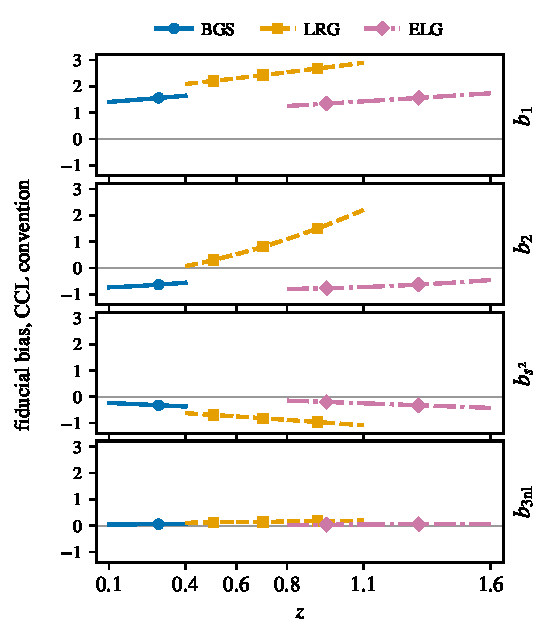
\includegraphics{plots/coevolution_biases/coevolution_biases.pdf}
\caption{The fiducial biases of the six DESI groups in the CCL
convention of Eq.~\eqref{eq:basis}, against redshift: the linear bias
$\bone = B_g/D(z)$, the Lazeyras et al. $\btwo$ of
Eq.~\eqref{eq:lazeyras}, and the co-evolution $\bs$ and $\bthree$ of
Eq.~\eqref{eq:coev}.  Each curve spans one group (the redshift ticks
are the group edges); the groups of one tracer share $B_g$, so their
curves join.  Markers sit at the DESI DR1 effective redshifts; ELG1,
which the DR1 full-shape analysis excluded, is marked near its group's
center.  $D$ is computed at the figure setup A of
Section~\ref{sec:fiducial} (Appendix~\ref{app:numerics}).}
\label{fig:coev}
\end{figure}

\subsection{Redshift space}
\label{sec:redshift-space}

In redshift space the one-loop model gains no new bias parameters but
several new terms.  The DESI DR1 methodology paper \cite{DESI2024V}
writes every full-shape model in the generic form
\begin{equation}
P_{s,g}(k,\mu) = P^{\rm PT}_{s,g}(k,\mu)
 + \left(\alpha_0 + \alpha_2\mu^2 + \alpha_4\mu^4\right) k^2
   \plin(k,\mu)
 + \left(\SNz + \SNt\,k^2\mu^2 + \mathrm{SN}_4\,k^4\mu^4\right) .
\label{eq:desi-generic}
\end{equation}
$P^{\rm PT}_{s,g}$ is the one-loop redshift-space spectrum of biased
tracers.  Its tree-level limit is the Kaiser spectrum
$(\bone + f\mu^2)^2\,\plin$; at one loop every bias operator of
Eq.~\eqref{eq:lagbasis} couples to the velocity field, producing
$\mu$-dependent loop terms with the same four bias coefficients
\cite{ChenVlahWhite2020,Maus2024}.  The counterterms
$\alpha_0,\alpha_2,\alpha_4$ absorb the small-scale sensitivity of the
loop integrals and the leading velocity dispersion; velocileptors
normalizes them as fractional corrections to the linear terms they
multiply, so that $\alpha_n = 12.5\aunit$ is a $50\%$ correction at
$k = 0.2\hMpc$ \cite{Maus2024}.  The stochastic terms descend from the
noise field: $\SNz$ is the deviation of the constant noise from the
Poisson value, $\SNt$ the velocity-weighted noise (the leading
Fingers-of-God stochastic term) and $\mathrm{SN}_4$ its next moment.
A projected analysis keeps the same biases;
Section~\ref{sec:projection} shows which $\mu$-dependent members
survive the projection into thin bins.

\section{The DESI DR1 full-shape model and priors}
\label{sec:desi}

The DESI DR1 full-shape analysis \cite{DESI2024V,DESI2024VII} fits the
power spectrum monopole and quadrupole of six tracer bins (BGS at
$z_{\rm eff}=0.295$, LRG1--3 at $0.510$, $0.706$, $0.919$, ELG2 at
$1.317$, QSO at $1.491$) over $0.02 < k < 0.2\hMpc$.  The ELG1 bin
($0.8<z<1.1$) failed the fibre-collision systematics tests and is
excluded from the full-shape analysis \cite{DESI2024V}.  The baseline
theory is the Eulerian mode of velocileptors, validated against Folps,
PyBird and a Gaussian-streaming configuration-space model
\cite{DESI2024V}.  The choices that matter here:

\begin{itemize}
\item \textbf{Basis and sampling.}  Even in the Eulerian mode, DESI
samples the Lagrangian parameters of Eq.~\eqref{eq:lagbasis},
reparameterized as the ``physical'' combinations
\begin{equation}
\left(1+\boneL\right)\sigma_8(z_{\rm eff}) , \qquad
\btwoL\,\sigma_8^2(z_{\rm eff}) , \qquad
\bsL\,\sigma_8^2(z_{\rm eff}) ,
\label{eq:physical-basis}
\end{equation}
because the data constrain these products directly and the
reparameterization reduces projection effects on $\sigma_8$
\cite{DESI2024V,DESI2024VII}.  $1+\boneL$ is the Eulerian linear bias,
so the first combination is $\bone\sigma_8(z_{\rm eff})$.
\item \textbf{Priors.}  Uniform $[0,3]$ on $(1+\boneL)\sigma_8$;
Gaussian with mean zero and width 5 on $\btwoL\sigma_8^2$ and on
$\bsL\sigma_8^2$; Gaussian with mean zero and width $12.5\aunit$ on
$\alpha_0$ and $\alpha_2$ (the $50\%$-correction-at-$\kmax$ rule);
Gaussian widths of 2 Poisson units on $\SNz$ and of 5 units of
$f_{\rm sat}\sigma_{\rm sat}^2/\bar{n}$ on $\SNt$, where $f_{\rm sat}$
is the satellite fraction and $\sigma_{\rm sat}$ the satellites'
velocity dispersion in distance units \cite{DESI2024V,DESI2024VII}.
\item \textbf{Fixed parameters.}  $\bthreeL = 0$, because the cubic
bias is expected to be small for intermediate-mass halos and is
degenerate with the counterterms \cite{DESI2024V,Maus2024};
$\alpha_4$ and $\mathrm{SN}_4$ drop with the hexadecapole, which DESI
DR1 does not fit.  The tidal bias is left free rather than tied to
co-evolution: tying it would add cosmological information that DESI
chose not to claim \cite{DESI2024V}.
\item \textbf{Budget.}  Seven nuisance parameters per tracer
($\boneL,\btwoL,\bsL,\alpha_0,\alpha_2,\SNz,\SNt$), 42 in total, with
the counterterms and stochastic terms marginalized analytically
\cite{DESI2024VII}.
\end{itemize}

Semenaite et al. \cite{Semenaite2025} fit the same DESI DR1 tracers in
configuration space jointly with weak lensing, with both tidal biases
fixed to calibrated relations in $\bone$ (the excursion-set
$\gamma_2(\bone)$ and the conserved-evolution
$\gamma_{21}(\bone,\gamma_2)$) and $\bone$ and $\btwo$ free per tracer.
Their mocks show that fixing the tidal sector to these relations
recovers unbiased cosmology for DESI-like tracers: direct evidence for
the calibration-anchored tidal bias of the model of
Section~\ref{sec:model}.

\section{The draft paper's bias table: the tidal-bias verdict}
\label{sec:verdict}

The draft paper's bias table (``bias parameters per DESI redshift
bin'') lists, per group, values labeled $b_1^{\rm E}$, $b_2^{\rm E}$,
$b_s^{\rm E}$, attributed to the DESI DR1 full-shape analysis.  Its
$b_s^{\rm E}$ column (positive, $0.6$--$1.4$) contradicts co-evolution,
which predicts $\bs$ between $-0.3$ and $-1.0$ for these tracers
(Figure~\ref{fig:coev}).  The numbers themselves establish where the
table comes from.

\begin{figure}[tbp]
\centering
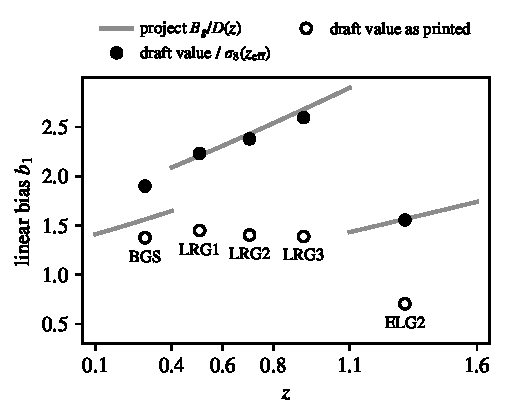
\includegraphics{plots/draft_bias_check/draft_bias_check.pdf}
\caption{The draft table's linear-bias column (``$b_1^{\rm E}$'')
read as the DESI physical combination $\bone\sigma_8(z_{\rm eff})$:
as printed (open circles) and divided by $\sigma_8$ at the group's
DESI DR1 effective redshift (filled circles), against the project's
fiducial $\bone = B_g/D(z)$ over each group (gray).  $\sigma_8(z)$ is
computed at the figure setup A of Section~\ref{sec:fiducial} (massless
neutrinos, $\sigma_8(0) = 0.843$).  The draft has no ELG1 row.}
\label{fig:draft-check}
\end{figure}

Three facts identify the table as the DESI physical-basis combinations
of Eq.~\eqref{eq:physical-basis} inserted raw:

\begin{enumerate}
\item \textbf{The linear column divided by $\sigma_8(z_{\rm eff})$
lands on the known biases for four of the five groups.}
Figure~\ref{fig:draft-check} shows the check: for LRG1--3 and ELG2 the
implied Eulerian bias agrees with the project's fiducial
$B_g/D(z_{\rm eff})$ to $1$--$3\%$.  An independent check at a
Planck-like cosmology ($\Omega_m = 0.3138$, $\sigma_8 = 0.8076$) finds
the same pattern, with ratios of $1.055$, $1.022$, $1.011$ and $1.038$.
Read directly as Eulerian biases, the column would make the three LRG
groups nearly unbiased ($\bone \simeq 1.4$ where LRGs sit near
$2.2$--$2.7$) and ELG2 anti-biased ($\bone = 0.70$) at $z = 1.3$.  The
BGS row is the exception: it implies $\bone \simeq 1.90$ against the
project's $1.56$, a ratio of $1.22$ ($1.27$ in the Planck-like check).
Whether that reflects the project's BGS amplitude $B_g = 1.34$, which
comes from the source forecast's configuration rather than a DESI DR1
fit, or a different origin of the row is not established; the BGS
entry of the public DESI DR1 chains decides it.
\item \textbf{The empty ELG1 row.}  DESI DR1 excluded ELG1 from the
full-shape analysis (Section~\ref{sec:desi}), so a table transcribed
from its products has nothing to put there.
\item \textbf{The magnitudes of the other two columns.}  Read as
$\btwoL\sigma_8^2$ and $\bsL\sigma_8^2$, the second and third columns
($-1.5$ to $+0.3$ and $+0.6$ to $+1.4$) sit inside the DESI Gaussian
priors of width 5 on exactly those combinations.  Read as CCL Eulerian
parameters they contradict both co-evolution and the DESI prior
centering.
\end{enumerate}

\textbf{Verdict.}  The draft's bias table holds the DESI DR1 sampling
combinations $(1+\boneL)\sigma_8(z_{\rm eff})$, $\btwoL\sigma_8^2$ and
$\bsL\sigma_8^2$, used as CCL's Eulerian $(\bone,\btwo,\bs)$ without
three transformations: removing the $\sigma_8$ powers, rotating the
Lagrangian parameters to the Eulerian basis with
Eq.~\eqref{eq:full-conversion}, and the factor of two between the
velocileptors and CCL tidal normalizations.  The linear column
establishes the reading for LRG1--3 and ELG2, and the table's
construction extends it to the other two columns.  The sign puzzle
dissolves: the column was never an Eulerian tidal bias.  The cost of
the raw reading is large.  The tidal term enters with the opposite
sign and several times the co-evolution magnitude (the BGS $\bone\bs$
product is $+1.96$ against $-0.50$), the quadratic coefficient differs
at a comparable level, and the loop sum moves by several percent of
$P_{gg}$ at $k \simeq 0.1\hMpc$, the size of the whole correction.  The
linear column, read as an Eulerian bias, is $30$--$55\%$ low for the
LRG and ELG groups: a free amplitude absorbs that in a fit, but a data
vector, a covariance or a Fisher derivative at a fixed fiducial carries
it.  The conversion, with the bracketed quantities DESI chain values
and $\sigma_8$ at the DESI fiducial cosmology, is
\begin{equation}
\bone = \frac{[(1+\boneL)\sigma_8]}{\sigma_8(z_{\rm eff})} , \quad
\btwo = \frac{[\btwoL\sigma_8^2]}{\sigma_8^2(z_{\rm eff})}
 + \frac{8}{21}\left(\bone - 1\right) , \quad
\bs = \frac{2\,[\bsL\sigma_8^2]}{\sigma_8^2(z_{\rm eff})}
 - \frac{4}{7}\left(\bone - 1\right) .
\label{eq:recipe}
\end{equation}
Applied to the draft's numbers it gives $\bsL \simeq 2.5$--$3.3$ and
$\bs \simeq +4$ to $+6$: chain values dominated by the width of the
DESI prior and by degeneracies with the counterterms, not a measurement
of the tidal field.  The model therefore imports no DESI nuisance
value: its fiducials are the calibrated relations of
Section~\ref{sec:coevolution}, and the DESI posteriors motivate only
its prior widths.

\section{The size of every term}
\label{sec:sizes}

Figure~\ref{fig:sizes} draws each one-loop term of Eq.~\eqref{eq:pgg}
in percent of the linear-bias model $\bone^2\pnl$, for four DESI-like
tracers at the calibrated biases of Figure~\ref{fig:coev}
(Appendix~\ref{app:numerics} gives the setup).
Figure~\ref{fig:poisson} shows, on the same scale, the Poisson power of
the project's thin bins, which the covariance carries as noise and
which sets the scale of the stochastic freedom.

\begin{figure}[tbp]
\centering
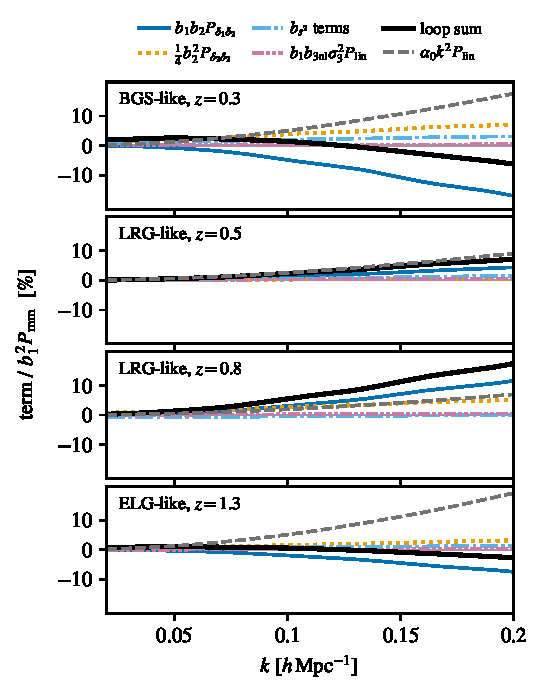
\includegraphics{plots/term_sizes/term_sizes.pdf}
\caption{Each one-loop term of Eq.~\eqref{eq:pgg} in percent of the
linear-bias model $\bone^2\pnl$ (halofit), against $k$ at the tracer
redshift, for four DESI-like tracers at the calibrated biases of
Figure~\ref{fig:coev}.  The three tidal terms
($\bone\bs P_{\delta_1 s_2}$, $\tfrac12\btwo\bs P_{\delta_2 s_2}$ and
$\tfrac14\bs^2 P_{s_2 s_2}$) are drawn as their sum.  Loop templates
are FAST-PT at $z=0$ scaled by $D^4(z)$, with the low-$k$ constants
kept (CCL's default, \texttt{sub\_lowk} off).  The dashed curve is the
counterterm $\alpha_0 k^2\plin(k,z)$ at DESI's width,
$\alpha_0 = 12.5\aunit$.}
\label{fig:sizes}
\end{figure}

\begin{figure}[tbp]
\centering
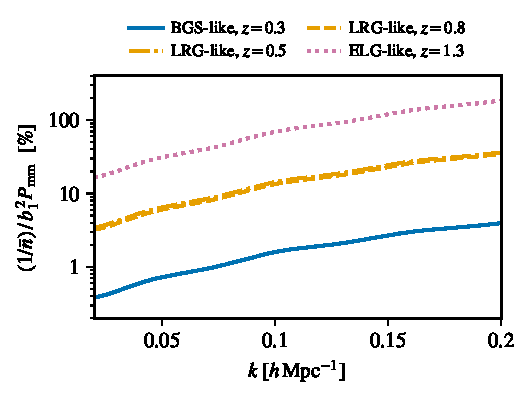
\includegraphics{plots/poisson_power/poisson_power.pdf}
\caption{The Poisson power $1/\bar{n}$ in percent of the linear-bias
model $\bone^2\pnl$ (halofit) of the four tracers of
Figure~\ref{fig:sizes}, with $\bar{n}$ the density of the project's
thin bin nearest each tracer redshift.  The covariance carries this
power as noise; it is drawn to set the scale of the stochastic
freedom.}
\label{fig:poisson}
\end{figure}

\paragraph{At model A's cut.}
Model A cuts each bin at $0.075\hMpc/D(\bar{z}_i)$: $0.088$, $0.097$,
$0.112$ and $0.139\hMpc$ for the four tracers of the figure.  At its
own cut the loop sum of each tracer is $+1.8\%$ (BGS-like), $+2.2\%$
and $+6.7\%$ (LRG-like at $z = 0.5$ and $0.8$) and $-0.4\%$
(ELG-like, where terms of $\pm4\%$ cancel); the largest single term is
the $\bone\btwo$ loop in every case.  The figure keeps the low-$k$
constants.  In CosmoLike's subtracted convention the BGS-like and
ELG-like sums become $-5\%$ and $-6\%$ and the LRG-like ones move by
under a point; the difference is white noise, carried by the
subtraction and by $\SNz$, not a change of shape.  The $\bone\bthree$
term stays below $0.3\%$ at $k \le 0.1\hMpc$.  Thirty percent of the
Poisson power, the non-Poisson stochasticity Nicola et al.
\cite{Nicola2023} detect in red samples, is $4$--$5\%$ of $P_{gg}$ for
the LRG-like tracers at their cuts and $31\%$ for the ELG-like tracer,
whose Poisson power there exceeds its clustering power.  Against the
forecast's sub-percent amplitude precision per group, none of these
is negligible.  Below the cut their scale dependence is mild, so the
linear amplitudes absorb most of each term and what remains is the
residual shape: the case for calibration-centered freedom with modest
priors, model A.

\paragraph{At the shipped mask.}
Model B's reference cut, the shipped mask, stops every bin at
$k = 0.176\hMpc$.  There the $\bone\btwo$ term alone is $4$--$14\%$ of
$P_{gg}$, with strong scale dependence, the loop sum reaches $15\%$
(LRG-like at $z = 0.8$), and the counterterm at DESI's width is
$6$--$15\%$.  No amplitude absorbs these terms, and their shapes
differ from one another: the case for model B's wider offsets and its
radial counterterm, the freedom DESI DR1 carries with seven nuisances
per tracer at $\kmax = 0.2\hMpc$.

\section{The model as implemented}
\label{sec:model}

\subsection{One likelihood option, every term per bin}
\label{sec:option}

The DESI likelihood (\texttt{likelihood/desi\_cl.py}) runs the one-loop
model when its option \texttt{higher\_order\_bias} is 1 (0 is linear
bias).  Every term is per bin.  The galaxy power of bin $i$ in redshift
space is
\begin{align}
P_{g,i}(k,\mu) ={}& P_{gg,i}(k)
 + \left(2\,b_{1,i}\,f\mu^2 + f^2\mu^4\right)\plin(k)
 + \left(b_{1,i} + f\mu^2\right) f\,\alpha_{2,i}\,\mu^2 k^2\,\plin(k)
 \nonumber\\
&+ \frac{1}{\bar{n}_i}\left(\mathrm{SN}_{0,i}
 + \mathrm{SN}_{2,i}\,f_{\rm sat}\sigma_{\rm sat}^2\,k^2\mu^2\right) ,
\label{eq:model}
\end{align}
whose real-space part is Eq.~\eqref{eq:pgg} in the subtracted
convention, with $\bthree = 0$ and the counterterm written on $\pnl$:
\begin{equation}
P_{gg,i}(k) = b_{1,i}^2\,\pnl(k)
 + P_{\rm loop}(k;\, b_{1,i}, b_{2,i}, b_{s^2,i})
 + \alpha_{0,i}\,k^2\,\pnl(k) ,
\label{eq:model-real}
\end{equation}
with $P_{\rm loop}$ the five quadratic templates of Eq.~\eqref{eq:pgg}.
Redshift-space distortions are linear (Kaiser) apart from the
$\alpha_2$ term, and each bin's redshift distribution is convolved
with the sampled Fingers-of-God dispersion $\sigma_v$, as in the
linear-bias model.  The terms:
\begin{itemize}
\item \textbf{Quadratic and tidal biases} follow each bin's own linear
bias through the calibrations of Section~\ref{sec:coevolution}, plus
offsets:
\begin{equation}
b_{2,i} = \btwo^{\rm fit}(b_{1,i}) + \Delta_{2,i} , \qquad
b_{s^2,i} = -\frac{4}{7}\left(b_{1,i} - 1\right) + \Delta_{s,i} .
\label{eq:perbin-evolution}
\end{equation}
Section~\ref{sec:evolution} explains why the relations take the full
$b_{1,i}$ and how the offsets are grouped.
\item \textbf{$\bthree = 0$}, DESI's baseline.  The co-evolution value
it discards, $|\bthree| \le 0.17$, is worth at most $0.3\%$ of
$P_{gg}$ at $k \le 0.1\hMpc$ (Figure~\ref{fig:sizes}) and is close in
shape to the counterterm; CosmoLike's $\bthree$ template is also
unusable (Appendix~\ref{app:open}).
\item \textbf{The counterterm $\alpha_0$}, in $h^{-2}\mathrm{Mpc}^2$,
rides CosmoLike's derivative-bias slot $2\,\bone b_K k^2\pnl$, with
$b_K = \alpha_0/[2\bone (c/H_0)^2]$ and $c/H_0 = 2997.92\Mpch$, because
CosmoLike measures $k$ in units of $H_0/c$.  The term multiplies
$\pnl$, where DESI's $\alpha_0$ multiplies $(\bone + f\mu^2)\bone\plin$:
the two coefficients differ by a factor $\bone^2$ and by the ratio
$\pnl/\plin$, at most $1.16$ at $k \le 0.2\hMpc$ for the tracers of
Figure~\ref{fig:sizes}.
\item \textbf{The radial counterterm $\alpha_2$}, in
$h^{-2}\mathrm{Mpc}^2$, follows the DESI DR1 field convention
\cite{Maus2024}: the galaxy density gains
$\tfrac12 f\mu^2\alpha_2 k^2\delta_{\rm L}$, with $\delta_{\rm L}$ the
linear density contrast, and twice its cross with the Kaiser field
$(\bone + f\mu^2)\delta_{\rm L}$ is the $\alpha_2$ term of
Eq.~\eqref{eq:model}.  The likelihood passes $\alpha_{2,i}$; the C code
(\texttt{galpha2} in \texttt{bias.c}) applies $b_{1,i}$ and $f$.
\item \textbf{The white noise $\SNz$}, in units of the bin's Poisson
power $1/\bar{n}_i$: the deviation from Poisson, since the covariance
carries the Poisson part.  $\bar{n}_i$ is fixed by the bin's surface
density, so that $1/\bar{n}_i$ projected with the raw redshift
distribution is the angular shot noise.
\item \textbf{The line-of-sight stochastic term $\SNt k^2\mu^2$}, in
units of $f_{\rm sat}\sigma_{\rm sat}^2/\bar{n}_i$, with the DESI DR1
values \cite{Maus2024} $(f_{\rm sat}, \sigma_{\rm sat}) =
(0.1, 7.8\Mpch)$ for LRG and $(0.1, 2.9\Mpch)$ for ELG; $\sigma_{\rm
sat}$ is not the Fingers-of-God $\sigma_v$.  BGS, absent from DESI's
table, takes the LRG values, a choice without consequence
(Section~\ref{sec:stochastic-projection}).
\end{itemize}
The compiled code has no stochastic slot, so the likelihood adds $\SNz$
and $\SNt$ as exact templates (Section~\ref{sec:stochastic-projection}).
A zero amplitude switches a term off at no cost: $\alpha_2 = 0$ in
every bin skips the term in the C code, and a stochastic family whose
amplitudes all vanish is not computed.  Of Eq.~\eqref{eq:desi-generic}
the model drops $\alpha_4$ and $\mathrm{SN}_4$, which DESI DR1 drops
with the hexadecapole, and the redshift-space one-loop terms, which
CosmoLike does not have (Appendix~\ref{app:open}); the derivative bias
$b_{\nabla^2}$ is exactly degenerate with $\alpha_0$ at one loop.

\paragraph{Why $\alpha_2$ takes DESI's field convention.}
In that convention $\alpha_2 k^2$ is a fractional correction: the
$\alpha_2$ term is $\alpha_2 k^2$ times the share of the Kaiser power
carried by the velocity term, $(\bone + f\mu^2) f\mu^2\plin$, whatever
the bias and the growth rate.  A prior width of $0.5/\kmax^2$ is then
a $50\%$ correction at $k = \kmax$ in every bin, the meaning of DESI's
$12.5\aunit$ at $0.2\hMpc$.  Written as a bare power,
$\alpha_2\mu^2 k^2\plin$, the same width would be a correction whose
size changes with $b_{1,i}$ and $f$ from bin to bin.

\subsection{Bias evolution within a group}
\label{sec:evolution}

The linear sector is the per-bin bias of the correlated-prior note
(its memory model).  Bin $i$ of group $g$ has
\begin{equation}
b_{1,i} = \frac{B_g\,(1 + \delta_i)}{D(\bar{z}_i)} , \qquad
\delta_i = s_g\,(\bar{z}_i - \bar{z}_g) + \varepsilon_i ,
\label{eq:linear-perbin}
\end{equation}
with $B_g$ the group amplitude, $\bar{z}_g$ the mean redshift of the
group's bins, $\delta_i$ the fractional deviation from the growth-tied
trend $B_g/D$, $s_g$ a free tilt, and $\varepsilon_i$ a residual under
a Gaussian prior correlated within the group,
\begin{equation}
\bigl\langle \varepsilon_i\,\varepsilon_j \bigr\rangle
 = \sigma_g^2\,\exp\!\left(-\,\frac{|\bar{z}_i - \bar{z}_j|}{L}\right) ,
\label{eq:kernel}
\end{equation}
and zero across groups; $\sigma_g$ is the per-bin width and $L$ the
correlation length in redshift.  The four linear-bias priors are
growth-tied ($\delta_i = 0$), baseline ($\sigma_g = 3\%$ for BGS and
$1\%$ elsewhere, $L = 0.2$), pessimistic ($3\%$ everywhere,
$L = 0.05$) and free (one flat bias per bin); the correlated-prior note
derives them.

The calibrations of Eq.~\eqref{eq:perbin-evolution} take the full
$b_{1,i}$, deviations included, not the smooth trend $B_g/D(\bar{z}_i)$.
A deviation $\delta_i$ is a real change of which halos the selection
reaches in that bin (a flux limit keeps only the brighter galaxies,
which sit in more massive halos), and the calibrations map halo
populations at a given linear bias, so the second-order biases of the
bin's population sit on the calibration curves at $b_{1,i}$.  The
induced shift is small but determined: near $\bone \simeq 2$ the
Lazeyras relation has slope $d\btwo/d\bone \simeq 1.7$, so a $3\%$
residual moves $\btwo$ by about $0.10$, a tenth of model A's offset
width, and the co-evolution slope $-4/7$ moves $\bs$ by about $0.03$.

The deterministic part carries the within-group evolution, which is
not small: across LRG3 the co-evolution $\bs$ moves from $-0.88$ to
$-1.09$ (Figure~\ref{fig:coev}), a drift comparable to the offset
width.  Holding $\btwo$ and $\bs$ constant across a group while
$b_{1,i}$ evolves would be inconsistent.  Freeing them per bin, 152
parameters on the $62$\,Mpc layout, is a bound rather than a model: a
bin's loop terms are nearly degenerate with its linear bias and
counterterm, so the prior would set the per-bin posteriors.

What a free parameter adds on top of the inherited trend is a drift of
the calibration itself: $\btwo$ at fixed $\bone$ changes with the
satellite fraction and the color mix, slowly within one selection.  The
freedom therefore sits per group.  Models A and B give each group one
offset, $\Delta_{2,i} = \Delta_{2,g}$ (and likewise $\Delta_s$);
\emph{model A + tilts} and \emph{model B + tilts} add a free straight
line in redshift within the group, the kind of line $s_g$ gives the
linear bias,
$\Delta_{2,i} = \Delta_{2,g} + t_{2,g}(\bar{z}_i - \bar{z}_g)$, with a
flat prior on the tilt $t_{2,g}$.  The counterterms follow the same
pattern, because their scale follows the size of the host halos, a population
property that drifts with the selection.  The stochastic amplitudes
never tilt: the Poisson part $1/\bar{n}_i$ is known per bin and sits in
the covariance, so only the non-Poisson fraction could drift, and
only what has a physical driver tilts.

\subsection{Models A and B}
\label{sec:models}

Models A and B are two parameter files of the one option, one per
layout and variant under \texttt{likelihood/}, written by
\texttt{scripts/make\_desi\_params.py} (options \texttt{--model-a} and
\texttt{--model-b}); the example yamls
\texttt{EXAMPLE\_EVALUATE\_MODEL\_A1}--\texttt{A4} and
\texttt{B1}--\texttt{B4} set them up on the four layouts.  The
likelihood reads every parameter per bin; a group is a yaml statement
that ties its bins to one offset, or to an offset and a tilt.
Table~\ref{tab:widths} lists the prior widths.  Either model, with or
without tilts, runs under any of the linear-bias priors.

\begin{table}[tbp]
\centering
\small
\begin{tabular}{lll}
\toprule
per group & model A & model B \\
\midrule
offsets $\Delta_2$ / $\Delta_s$ & $1.0$ / $0.5$ & $2.0$ / $1.0$ \\
$\alpha_0$ [$h^{-2}\mathrm{Mpc}^2$] & $0.5/\kmax^2$ & $0.5/\kmax^2$ \\
$\alpha_2$ [$h^{-2}\mathrm{Mpc}^2$] & fixed to $0$ & $0.5/\kmax^2$ \\
$\SNz$ [$1/\bar{n}_i$] & $2$ & $2$ \\
$\SNt$ [$f_{\rm sat}\sigma_{\rm sat}^2/\bar{n}_i$] & $5$ & $5$ \\
tilted (+ tilts only) & $\Delta_2$, $\Delta_s$, $\alpha_0$
 & $\Delta_2$, $\Delta_s$, $\alpha_0$, $\alpha_2$ \\
parameters, without / with tilts & $5$ / $8$ & $6$ / $10$ \\
\bottomrule
\end{tabular}
\caption{The widths of the Gaussian priors of the higher-order
parameters, all centered on zero, and their number per group (the
tilts, with flat priors, only in groups of more than one bin).
$\kmax$ is the fit's cut, quoted at $z = 0$; each bin is cut at
$\kmax/D(\bar{z}_i)$.  Model A: $\kmax = 0.075\hMpc$, an $\alpha_0$
width of $88.9\aunit$.  Model B: each cut of a scan, or the shipped
mask, $0.176\hMpc$ in every bin ($16.1\aunit$).}
\label{tab:widths}
\end{table}

The widths have stated sources.
\begin{itemize}
\item \textbf{Offsets.}  Model A's $1.0$ and $0.5$ cover the known
imperfection of the calibrations: the scatter of the Lazeyras fit and
the $30\%$ spread between co-evolution and the excursion-set $\bs$ at
LRG biases.  Model B doubles them, demoting the calibrations to prior
centers for cuts where the loops reach $15\%$ of $P_{gg}$.
\item \textbf{Counterterms.}  The DESI rule of a $50\%$ correction at
the cut, evaluated at each cut: $0.5/\kmax^2$, which is DESI's $12.5$
at $0.2\hMpc$.  Because $\alpha_0$ multiplies $\pnl$, at bin $i$'s own
cut the width is a correction of $0.5/B_g^2$ of the linear galaxy power
$b_{1,i}^2\pnl$, the same in every bin of a group: $28\%$ for BGS,
$17\%$ for LRG, $71\%$ for ELG at model A's cut.
\item \textbf{Stochastic terms.}  DESI DR1's widths.
\end{itemize}

Model A is built for $\kmax = 0.075\hMpc$, the cut matched to the
thin-bin radial resolution.  It fixes $\alpha_2 = 0$: at DESI's width
the $\alpha_2$ term changes the kept auto spectra by about $1\%$
(Section~\ref{sec:rsd-projection}), and a fit without $\alpha_2$ holds
against a truth with $\alpha_2 = \pm12.5\aunit$
(\texttt{notes/fog\_parameter\_degeneracy\_study}).  Model A carries
$\SNt$ because without it the thin layouts fail at its cut
(Section~\ref{sec:stochastic-projection}).  Model B frees $\alpha_2$
for the scan in $\kmax$.  With the amplitude $B_g$ and the linear tilt
$s_g$, model B has eight parameters per group: DESI DR1's
seven per tracer \cite{DESI2024V,DESI2024VII} plus the linear tilt the
thin bins resolve.  Every fiducial higher-order parameter is zero, so
the fiducial model sits on the calibrations; no DESI chain value
enters (Section~\ref{sec:verdict}).

\subsection{The paper model}
\label{sec:papermodel}

The paper forecast runs one configuration of this option: model B +
tilts with $\alpha_2$ fixed to zero in every bin and every $\sigma_v$
prior width multiplied by six, on the pessimistic linear-bias prior.
Its example yamls are \texttt{EXAMPLE\_EVALUATE1}--\texttt{4}, built
on the parameter files
\texttt{params\_desi[\_<case>]\_bias\_pessimistic.yaml} (the
pessimistic linear bias) and
\texttt{params\_desi[\_<case>]\_model\_b\_tilts.yaml} (model B +
tilts with $\alpha_2 = 0$).
The sampled Fingers-of-God
dispersions reproduce the $\alpha_2$ derivative templates almost
exactly, so dropping $\alpha_2$ and widening the $\sigma_v$ priors
sixfold lets the dispersions absorb an $\alpha_2$ of DESI's size:
fitted to a truth with $\alpha_2 = \pm12.5\aunit$, the paper model
moves no scored parameter by more than $0.33\sigma$
(\texttt{notes/fog\_parameter\_degeneracy\_study} derives the factor
of six and the shifts).  Every other width is model B's
(Table~\ref{tab:widths}); Section~\ref{sec:fiducial} lists the
$\sigma_v$ fiducials and widths.

\subsection{The covariance}
\label{sec:covariance}

The Gaussian covariance is built on the one-loop fiducial:
$b_{1,i} = B_g/D(\bar{z}_i)$, $\btwo$ and $\bs$ on the calibrations,
every other term zero.  Models A and B, with or without tilts, share
that fiducial, so one covariance serves all of them.  Its one-loop terms come from CosmoLike's own
tables of C-FASTPT (its C port of FAST-PT), with the data vector's
bilinear pair form
(Section~\ref{sec:separability}), and enter through Limber; the low-$\ell$
non-Limber recompute stays linear (Appendix~\ref{app:open}).
\texttt{nonlimber\_accuracyboost} 2 converges the adjacent thin-bin
cross spectra to $2\%$ and the diagonal to $0.4\%$.  The covariance
takes massless neutrinos, so its signal sits $3\%$ above the data
vector ($m_\nu = 0.06$\,eV) at every redshift.  Against a linear-bias
covariance, the figures of merit move by $-0.4\%$ to $+1.2\%$.

\section{Projection to thin-bin angular spectra}
\label{sec:projection}

\subsection{Separability and the \texorpdfstring{$D^4$}{D\textasciicircum 4} rule}
\label{sec:separability}

The exact (non-Limber) angular power spectrum between bins $i$ and $j$
is
\begin{equation}
C_\ell^{ij} = \frac{2}{\pi} \int dk\,k^2
 \int d\chi_1\,W_i(\chi_1)\,j_\ell(k\chi_1)
 \int d\chi_2\,W_j(\chi_2)\,j_\ell(k\chi_2)\;
 \mathcal{P}\!\left(k; z_1, z_2\right) ,
\label{eq:cl}
\end{equation}
where $W_i(\chi)$ is the bin's radial kernel (the normalized,
Fingers-of-God-convolved redshift distribution expressed in comoving
distance $\chi$), $j_\ell$ is the spherical Bessel function, and
$\mathcal{P}$ is the unequal-time galaxy power spectrum.  Every term of
the one-loop expansion is separable in $k$ and time:
\begin{itemize}
\item the linear term carries $D(z_1)\,D(z_2)$;
\item the five quadratic templates are 22-type mode-coupling integrals
over two linear spectra, so each carries $D^2(z_1)\,D^2(z_2)$;
\item the 13-type pieces (the $\sigma_3^2\plin$ term of $\bthree$ and
the $P_{13}$ inside the one-loop matter spectrum) carry the symmetrized
$\tfrac{1}{2}\left[D^3(z_1)D(z_2) + D(z_1)D^3(z_2)\right]$.
\end{itemize}
At equal times every loop term scales as $D^4(z)$.  CCL, velocileptors
and CosmoLike all compute the templates once from the $z = 0$ linear
spectrum and rescale them by $D^4$ \cite{DESI2024VII}; CosmoLike's
\texttt{get\_FPT\_bias} (\texttt{pt\_cfastpt.c}) builds them with
C-FASTPT and rebuilds them when the cosmology changes.  For thin bins
the equal-time evaluation at the bin mean is accurate: across a
$\Delta z = 0.02$ bin the growth factor changes by about $1\%$, the
symmetric products differ from $D^4(z_{\rm mid})$ only at second order
in that $1\%$, and the residual is a few parts in $10^4$ of the loop
terms.

The auto spectrum of Eq.~\eqref{eq:pgg} is a quadratic form in the
bias vector $u_i = (b_{1,i}, b_{2,i}, b_{s^2,i})$,
$P_{gg,i} = u_i^{\mathsf T} Q\, u_i$, with $Q$ the symmetric matrix of
templates ($Q_{11} = \pnl$, $Q_{12} = \tfrac12 P_{\delta_1\delta_2}$,
$Q_{22} = \tfrac14 P_{\delta_2\delta_2}$, and so on).  A cross pair of
bins $i$ and $j$ carries the bilinear form $u_i^{\mathsf T} Q\, u_j$:
each product of two biases is shared between the two bins.  The
low-rank engine projects each bin's full one-loop $P_{gg,i}$,
counterterm included, through an SVD of its square root, so it carries
the one-loop sum with no structural change; for the cross pairs it
uses the bilinear form.

CosmoLike subtracts the low-$k$ constants of the quadratic templates
(Section~\ref{sec:realspace}), so the loop sum vanishes as $k \to 0$
and large scales keep the linear-bias spectrum.  As $k \to \infty$ the
templates decay and the subtraction leaves a constant,
\begin{equation}
P_\infty = -\frac{\sigma_4}{2}\,D^4(z)
 \left(\btwo + \frac{2}{3}\,\bs\right)^2 \le 0 ,
\label{eq:pinf}
\end{equation}
with $\sigma_4 = 4391\,(h^{-1}\mathrm{Mpc})^3$ at $z = 0$ at the
likelihood's fiducial.  Where this negative constant outweighs the
decaying positive terms, $P_{gg}$ turns negative at high $k$ and its
square root does not exist.  The low-rank engine handles the constant
exactly: it factorizes $P_{gg} - P_\infty$ and projects $P_\infty$
separately (Section~\ref{sec:whitenoise}).

\subsection{Linear redshift-space distortions and the counterterms}
\label{sec:rsd-projection}

Linear (Kaiser) redshift-space distortions enter Eq.~\eqref{eq:cl}
through the transformation of the density kernel: each factor of
$f\mu^2$ in the flat-sky spectrum becomes a second derivative of the
Bessel function in the exact projection,
\begin{align}
\Delta_\ell^i(k) &= \int d\chi\,W_i(\chi)
 \left[\bone(z)\,j_\ell(k\chi) - f(z)\,j_\ell''(k\chi)\right] D(z) ,
 \nonumber\\
R_\ell^i(k) &= -\int d\chi\,W_i(\chi)\,f(z)\,j_\ell''(k\chi)\,D(z) ,
\label{eq:kaiser}
\end{align}
with $\Delta_\ell^i$ the whole linear transfer of bin $i$ and
$R_\ell^i$ its velocity part.  For wide photometric bins the
$j_\ell''$ term integrates down by orders of magnitude; for shells
thinner than the scales probed it survives at full strength, because
the shell resolves line-of-sight modes with $\mu$ near one.  This is
why thin-bin $C_\ell^{gg}$ recovers the Kaiser information of a
three-dimensional analysis \cite{Asorey2012}, and it cuts both ways:
every $\mu$-dependent term that a wide-bin analysis could drop is
alive here.

\paragraph{$\alpha_0$.}  The $\alpha_0$ term is $\mu$-independent and
projects like the density: one extra $k$-shape, $k^2\pnl$, in each
bin's $P_{gg,i}$.  The engine matters.  FKEM, the FFTLog method of
Fang et al. \cite{FangKEM2020}, projects only the linear term exactly
and moves every nonlinear term, the counterterm included, through its
Limber difference; the low-rank engine projects the
counterterm without the Limber approximation.  On the $\Delta z = 0.05$
layout the low-rank $\alpha_0$ response is $7.3$ times the Limber one
at $\ell = 20$ and $1.26$ times at $\ell = 100$, from the $k^2$-weighted
radial modes of thin, sharp-edged bins, so the model runs on the
low-rank engine (the correlated-prior note,
\texttt{notes/correlated\_bias\_prior\_v2}, on why the counterterm
requires the low-rank engine).

\paragraph{$\alpha_2$.}  The counterterm field of bin $i$,
$\tfrac12 f\mu^2\alpha_{2,i} k^2\delta_{\rm L}$, has the transfer
$\tfrac12\alpha_{2,i}k^2 R_\ell^i$, and its cross with the linear field
of bin $j$ adds
\begin{equation}
\Delta C_\ell^{ij} = \frac{2}{\pi}\int dk\,k^2\,\plin(k)\,
 \frac{k^2}{2}\left[\alpha_{2,i}\,R_\ell^i\,\Delta_\ell^j
 + \alpha_{2,j}\,\Delta_\ell^i\,R_\ell^j\right] ,
\label{eq:alpha2-proj}
\end{equation}
which for an auto spectrum is $\alpha_{2,i}k^2\Delta_\ell^i R_\ell^i$
under the integral.  The projection reuses the two transfers the
Kaiser term already builds, adds no Bessel integral, and is exact;
every gg engine carries it (FFTLog, low-rank, FKEM pairs, and Limber
with $\plin$).  It is linear in $\alpha_2$ to $10^{-12}$, and a
brute-force $j_\ell$, $j_\ell''$ double integral agrees with it to
$6\times10^{-4}$ for a thin auto spectrum and an adjacent pair at
$\ell = 2$--$500$.  At DESI's width, $12.5\aunit$, it raises the auto
spectra of the shipped mask by a median $0.7\%$ ($\Delta z = 0.05$)
and $1.1\%$ ($\Delta d_{\rm com} = 62$\,Mpc), at most $2.9\%$.

The Fingers-of-God convolution of each bin's redshift distribution is a
nonperturbative stand-in for part of the same physics: it damps radial
power with a shape set by the sampled $\sigma_v$, and is partially
degenerate with $\alpha_2$.  Partial degeneracy is not identity: the
convolution is a positive damping of fixed functional form, while
$\alpha_2$ takes either sign and scales as $k^2\plin$.

\subsection{Stochastic terms in projection}
\label{sec:stochastic-projection}

A constant three-dimensional power $N$ projects to
\begin{equation}
C_\ell^{ij}\big|_{\rm stoch}
 = N \int d\chi\, \frac{W_i(\chi)\,W_j(\chi)}{\chi^2} ,
\label{eq:sn-projection}
\end{equation}
independent of $\ell$.  Equation~\eqref{eq:sn-projection} is exact,
not a Limber approximation: for a constant $\mathcal{P}$ the $k$
integral of Eq.~\eqref{eq:cl} collapses by Bessel orthogonality, so
the Limber formula is exact for white noise.  For a top-hat bin of
width $\Delta\chi$ the result is $N/(\chi^2\Delta\chi)$, and at the
Poisson value $N = 1/\bar{n}$ it reproduces the angular shot noise
$1/\bar{n}_{2D}$, with $\bar{n}_{2D}$ the surface density of the bin.
The model's $\SNz$ templates are Eq.~\eqref{eq:sn-projection} with the
Fingers-of-God-convolved kernels, which overlap for adjacent thin bins,
so a stochastic term also reaches the measured cross spectra.  A cross
pair within one tracer sample takes the mean of the two bins' Poisson
powers; a pair of two samples (an LRG and an ELG bin at the same
redshift) takes none, because different galaxies share no stochastic
term.

\paragraph{$\SNt$ projects exactly too.}  A power proportional to
$k^2\mu^2 = k_\parallel^2$ is that of the radial derivative
$\partial_\chi\epsilon$ of a white noise $\epsilon$.  Projected with
the kernel of bin $i$, $\int d\chi\,W_i\,\partial_\chi\epsilon =
-\int d\chi\,W_i'\,\epsilon$ (integration by parts, with
$W_i' = dW_i/d\chi$ and the kernel vanishing at its ends), so the
$\SNt$ term is Eq.~\eqref{eq:sn-projection} with each kernel replaced
by its radial derivative:
\begin{equation}
C_\ell^{ij}\big|_{\SNt} = U_{ij} \int d\chi\,
 \frac{W_i'(\chi)\,W_j'(\chi)}{\chi^2} ,
\qquad U_i = \frac{\mathrm{SN}_{2,i}\,f_{\rm sat}\sigma_{\rm sat}^2}{\bar{n}_i} ,
\label{eq:sn2-projection}
\end{equation}
with $U_{ij}$ the mean of $U_i$ and $U_j$ within one sample and zero
across samples.  A thin bin's kernel is a top hat smoothed only by the
Fingers-of-God convolution, so $W_i'$ peaks at the two edges, positive
on the rising edge and negative on the falling one.  The sharper the
edges, the larger the template: per unit, the $\SNt$ auto template is
a median $0.022$, $0.017$, $0.0065$ and $0.0017$ times the $\SNz$ one
on the $62$\,Mpc, $\Delta z = 0.02$, $0.05$ and $0.2$ layouts.

\paragraph{Neighbors are anticorrelated.}  Adjacent thin bins share an
edge: the falling edge of one is the rising edge of the next, so
$W_i'W_j' < 0$ there and the projected $\SNt$ of two neighbors is
negative.  On the $62$\,Mpc layout the normalized adjacent term,
$K_{ij}/\sqrt{K_{ii}K_{jj}}$ with $K_{ij}$ the integral of
Eq.~\eqref{eq:sn2-projection}, has a median of $-0.50$ over the 73
adjacent pairs, against $+0.05$ for $\SNz$.  A white noise adds only
positive cross terms, products of positive kernels, so no $\SNz$, per
group or per bin, reproduces the pattern.

\paragraph{Why model A carries $\SNt$.}  Without $\SNt$, a truth with
$\SNt = \pm5$ units, the one-sigma width of its prior, moved a model A
fit's
$\Omega_m$ by $1.3$--$1.7\sigma$ at $\kmax = 0.075\hMpc$ on the two
thin layouts, mostly through the adjacent cross spectra.  Model A then
held only to $0.05\hMpc$ on the $62$\,Mpc layout and failed at its
first fitted cut, $0.075\hMpc$, on $\Delta z = 0.02$.  The LRG term
carried the effect.  ELG alone moved $\Omega_m$ by at most
$0.23\sigma$ (its unit, $0.84\,(h^{-1}\mathrm{Mpc})^2$, is a seventh of
LRG's $6.08$), and BGS by $0.00$, with the borrowed LRG unit or with
one built from the BGS bins' own Fingers-of-God dispersion, so the BGS
unit does not matter.  With one $\SNt$ per group, model A holds to its
own cut on the thin layouts.  About half
of each bin's $\SNt$ auto kernel comes from $k_\parallel$ above the
bin's own cut at $\kmax = 0.075\hMpc$, a content the scale cut does
not weigh (Appendix~\ref{app:open}).

\subsection{The white-noise limit of the renormalized loops}
\label{sec:whitenoise}

\paragraph{Origin of the constant.}
The template $P_{\delta_2\delta_2}$ is the power spectrum of the
operator $\delta^2$.  Its four linear fields pair across the two
operators in two ways (two Wick contractions), and each pairing gives
$\int_{\mathbf{q}}\plin(q)\,\plin(|\mathbf{k}-\mathbf{q}|)$.  As
$k \to 0$ this integral tends to $\sigma_4 = \int_{\mathbf{q}}\plin^2(q)$,
so $P_{\delta_2\delta_2} \to 2\sigma_4$.  The constant comes from pairs
of nearly opposite wavevectors, $\mathbf{q}$ and
$\mathbf{k}-\mathbf{q} \simeq -\mathbf{q}$, whose sum is the long mode;
on scales much larger than $1/q$ it is indistinguishable from white
noise.  The tidal templates carry the kernel
$S_2 = \mu_{12}^2 - \tfrac{1}{3}$ of Appendix~\ref{app:loops}, which
equals $\tfrac{2}{3}$ for opposite wavevectors ($\mu_{12} = -1$): one
power of it gives $P_{\delta_2 s_2} \to \tfrac{4}{3}\sigma_4$, two give
$P_{s_2 s_2} \to \tfrac{8}{9}\sigma_4$.

Subtracting these constants renormalizes the operators: the constant
moves into the stochastic sector and the loops vanish on large scales.
As $k \to \infty$ the templates decay, so the subtracted loop sum of
Eq.~\eqref{eq:pgg} tends to minus the subtracted constants, each with
its bias coefficient:
\begin{equation}
\tfrac{1}{4}\btwo^2\,(2\sigma_4)
 + \tfrac{1}{2}\btwo\bs\,(\tfrac{4}{3}\sigma_4)
 + \tfrac{1}{4}\bs^2\,(\tfrac{8}{9}\sigma_4)
 = \frac{\sigma_4}{2}\left(\btwo + \tfrac{2}{3}\bs\right)^2 .
\label{eq:pinf-algebra}
\end{equation}
With the $D^4$ scaling, this square with a minus sign is $P_\infty$ of
Eq.~\eqref{eq:pinf}.  The perfect square has a reading:
$\btwo + \tfrac{2}{3}\bs$ is the quadratic coefficient in the Galileon
basis of Appendix~\ref{app:conversions}, and the Galileon kernel
$S_2 - \tfrac{2}{3} = \mu_{12}^2 - 1$ vanishes for opposite
wavevectors, so $\mathcal{G}_2$ adds no constant of its own.

\paragraph{Two conventions, one model.}
CosmoLike subtracts the three constants, as CCL does with
\texttt{sub\_lowk} on.  Velocileptors, in both its Eulerian and
Lagrangian flavors, keeps the loop proportional to the square of the
quadratic bias unsubtracted (in the Lagrangian flavor
$\tfrac{1}{2}(\btwoL)^2\xi_{\rm lin}^2$ in configuration space, with
$\xi_{\rm lin}$ the linear correlation function); it removes only the
operator means of Eq.~\eqref{eq:lagbasis}, which touch only the $k = 0$
mode, and its $\SNz$ absorbs the low-$k$ constant
\cite{ChenVlahWhite2020,Maus2024}.  The subtracted spectrum with $\SNz$
centered at zero equals the unsubtracted spectrum with $\SNz$ centered
at $-(\sigma_4/2)D^4(\btwo + \tfrac{2}{3}\bs)^2$, a center that moves
with the biases.  A prior on $\SNz$ with a fixed center therefore
states different physics in the two conventions.

\paragraph{Where $P_{gg}$ turns negative.}
Let $k_{\rm neg}$ be the wavenumber at which the subtracted one-loop
$P_{gg}$ first turns negative, and $\Delta_2 = \btwo - \btwo^{\rm
fit}(\bone)$ the offset of Eq.~\eqref{eq:perbin-evolution}.
Figure~\ref{fig:kneg} draws $k_{\rm neg}$ against $\Delta_2$ for three
representative bins.  In the LRG bins the constant stays small against
the galaxy power, because the calibrated $\btwo$ partly cancels
$\tfrac{2}{3}\bs$ and the larger $\bone^2$ raises the positive terms:
$k_{\rm neg} > 1.5\hMpc$.  At the calibrated biases ($\Delta_2 = 0$),
$|P_\infty|$ is $5$--$42$ times the Poisson power in the forecast's BGS
bins, where $1/\bar{n} \simeq 33$--$170\,(h^{-1}\mathrm{Mpc})^3$, and
$3$--$15\%$ of it in the ELG bins.  Only negative offsets matter:
$\btwo + \tfrac{2}{3}\bs$ vanishes near $\Delta_2 \simeq +0.9$, so a
positive offset shrinks the constant and pushes $k_{\rm neg}$ far out.

\begin{figure}[tbp]
\centering
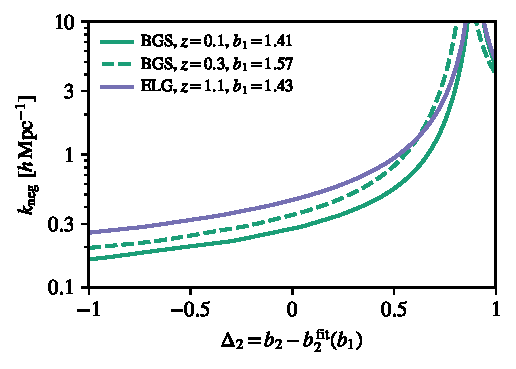
\includegraphics{plots/k_neg/k_neg.pdf}
\caption{The wavenumber $k_{\rm neg}$ at which the one-loop $P_{gg}$
in CosmoLike's subtracted convention first turns negative, against
the offset $\Delta_2$ of $\btwo$ from the Lazeyras calibration, for
two BGS bins and one ELG bin.  $\bs$ is on co-evolution,
$\bone = B_g/D(z)$, and $\bthree$ and the counterterm are zero.  The
leading term is $\bone^2 D^2\plin$; the halofit $\pnl$ of the model is
larger at these wavenumbers, so the model turns negative at somewhat
higher $k$.  Where $\btwo + \tfrac{2}{3}\bs$ vanishes, $P_\infty$
vanishes with it and $k_{\rm neg}$ leaves the panel.  Setup in
Appendix~\ref{app:numerics}.}
\label{fig:kneg}
\end{figure}

\paragraph{Why thin-bin angular spectra see it and DESI's fits do not.}
An angular spectrum integrates $P(k)$ over all $k$ through each bin's
radial window (Eq.~\eqref{eq:cl}).  A thin bin passes radial modes far
above the transverse wavenumber of a band, so no cut in $\ell$
excludes the region $k > k_{\rm neg}$; the UV-fraction cut only bounds
its share.  A white noise projects exactly
(Eq.~\eqref{eq:sn-projection}), so in the subtracted convention
$P_\infty$ enters every multipole at full strength.  DESI's full-shape
fits are spared both effects.  They use only $0.02 < k < 0.20\hMpc$ in
three dimensions \cite{DESI2024V}, and the DESI DR1 samples are sparse:
DR1 BGS holds 300{,}017 galaxies over $0.1 < z < 0.4$, which with the
survey area gives $1/\bar{n} \approx 3\times10^3\,(h^{-1}\mathrm{Mpc})^3$
(an estimate made for this note).  The constant is then at most of the
order of the Poisson power and fits DESI's $\SNz$ prior in either
convention.  The forecast's BGS is $20$--$100$ times denser.

\paragraph{What CosmoLike does.}
The low-rank engine splices its non-Limber density term into the
Limber spectrum: it takes the full Limber $C_\ell$, subtracts the
Limber projection of the density-only term, and adds the non-Limber
projection of the same term.  The white-noise constant passes through
this splice exactly:
\begin{itemize}
\item the engine factorizes $P_{gg} - P_\infty$, the spectrum with the
unsubtracted templates, which is positive, so its square root exists;
\item the Limber density-only term subtracted in the splice uses the
same unsubtracted templates;
\item the full Limber term keeps the subtracted templates, so
$P_\infty$ reaches $C_\ell$ through Limber, exact for a constant power;
\item a cross pair carries the bilinear constant
$-(\sigma_4/2)D^4(b_{2,i} + \tfrac{2}{3}b_{s^2,i})
(b_{2,j} + \tfrac{2}{3}b_{s^2,j})$.
\end{itemize}
A floor on the factorized spectrum stays in the code as a guard; the
tested vectors do not reach it.  Compared with flooring $P_{gg}$
instead, the exact treatment leaves linear-bias vectors and FKEM
one-loop vectors bitwise unchanged, as it must, and moves the low-rank
one-loop vector at the calibrated biases by at most $5\times10^{-3}$ of
the angular shot noise.  At the highest band model A keeps, the share of a bin's white-noise projection from
$k > k_{\rm neg}$ is at most $0.34\%$ (BGS, $z = 0.11$) and about zero
for ELG (a flat-sky estimate at the calibrated biases).  One model A
prior width below the calibrations ($\Delta_2 = -1$,
$\Delta_s = -0.5$), the exact treatment shows negative $C_\ell$ in the
lowest BGS bins beyond $k \approx 0.15\hMpc$ (Limber correspondence
$k = (\ell + \tfrac12)/\chi$) on the shipped mask, $-29$ times the shot
noise at $\ell = 50$ ($-25$ with FKEM, Limber in its one-loop content),
which a floor would hide.  At the model A cut the same biases keep
every kept $C_\ell$ positive, and the exact treatment moves them by at
most $0.27$ of the shot noise.

\paragraph{Consequences.}
Model A at $\kmax = 0.075\hMpc$ is safe: at the calibrated biases the
region beyond $k_{\rm neg}$ carries a negligible share of its kept
bands, and one prior width below the calibrations every kept $C_\ell$
stays positive.  At model B's higher cuts on the dense low-redshift
BGS, one-loop perturbation theory is not trustworthy near
$k \approx 0.15$--$0.2\hMpc$ once $\btwo$ sits a unit below the
calibration (Figure~\ref{fig:kneg}).  A Fisher forecast at the
fiducial is unaffected; chains that reach such points meet the open
issue of positivity (Appendix~\ref{app:open}).  Two levers miss the
sign problem: a tighter $\btwo$ prior only shifts $k_{\rm neg}$, and
$\SNz$ adds the same constant at every $k$.  The subtracted convention
is also why $\SNz$ keeps DESI's width in Poisson units: in the
unsubtracted convention $\SNz$ would have to absorb $5$--$42$ Poisson
units in the forecast's BGS, far outside a width of $2/\bar{n}$.

\section{Validation}
\label{sec:validation}

Each piece of the model was checked against an independent
calculation, and the forecast built on it was tested against truths it
does not contain.  The checks of the $\alpha_2$ projection and of the
white-noise splice are in Sections~\ref{sec:rsd-projection} and
\ref{sec:whitenoise}.
\begin{itemize}
\item \textbf{Loop templates.}  With $\bthree = 0$, CosmoLike's
C-FASTPT templates and Python FAST-PT agree to
$\Delta\chi^2 \le 3.5\times10^{-5}$ on the $62$\,Mpc vector, cross
pairs included.  Doubling the C-FASTPT grid moves $\Delta\chi^2$ by
$\sim10^{-8}$, raising \texttt{accuracyboost} to 3--4 moves the
one-loop part by $\Delta\chi^2 \le 4.5\times10^{-3}$, and the low-rank
rank is converged at 5 (5 to 12: $10^{-10}$).  One setting fails:
\texttt{internal\_accuracyboost} $= 4$ breaks the C-FASTPT bias tables
($\Delta\chi^2 \sim 10^{12}$).
\item \textbf{Cross pairs.}  The one-loop pair code leaves linear-bias
vectors bitwise unchanged with the low-rank, FKEM and Limber engines.  A pair of two bins with
identical redshift distributions equals the polarization of the auto
spectra (the bilinear form recovered from the quadratic one) to
$10^{-14}$ of the one-loop increment.  One and eight threads give
identical vectors.
\item \textbf{The likelihood option.}  A zero amplitude reproduces the
vector without the term bitwise.  The $\alpha_2$ and $\SNt$ terms are
linear (forward and backward differences of the $\alpha_2$ columns
agree to $3\times10^{-10}$ of the column; $\SNt$ to $3\times10^{-14}$),
and the stochastic-template code run at order zero reproduces the
$\SNz$ templates of the Fisher notebook's derivative caches exactly.
\item \textbf{The covariance.}  Its one-loop increment equals an
independent evaluation of the data-vector formula to $1.5\times10^{-13}$
(gg) and $3.2\times10^{-12}$ (gs), and its mean signal divided by the
one-loop fiducial data vector is flat at $1.03$, the massless-neutrino
offset.
\item \textbf{The derivatives.}  The per-bin bias columns of the Fisher
construction, summed through the chain rule of
Eq.~\eqref{eq:perbin-evolution}, reproduce the stencil derivative of
each group amplitude (the correlated-prior note, on its numerical
checks).
\item \textbf{The forecast.}  The correlated-prior note fits random
bias histories under every linear-bias prior (its accuracy test), and
the Fisher notebook of the paper model,
\texttt{EXAMPLE\_EVALUATE\_FISHER\_MODEL.ipynb}, fits model B and
model B + tilts to four fixed truths: $\alpha_2$ at one model B width
($0.5/\kmax^2$), $\SNt = \pm5$, the offsets at one sigma of model B's
widths, and a linear drift of the calibrations across each group
($\Delta_2$ changing by $1$ and $\Delta_s$ by $0.5$, with zero mean).
The first three lie inside model B's prior and are reported; the
drift is tested, and a model holds at a cut while every tested shift
stays below $\sigma/3$.  Model B on the baseline prior breaks at
$0.075\hMpc$ on the two thin layouts (the drift moves $(w_0, w_a)$ by
$0.82$ and $0.86\sigma$ at $0.1$) and at $0.05$ on $\Delta z = 0.05$
and $0.2$ ($0.35$ and $0.36\sigma$ at $0.075$).  Model B + tilts on
the pessimistic prior absorbs the drift exactly and passes every cut;
its reported in-prior shifts reach $0.98\sigma$ at $0.075$ on
$\Delta d_{\rm com} = 62$\,Mpc and $1.10\sigma$ at $0.1$ on
$\Delta z = 0.02$, both from $\alpha_2$.  The paper model
(Section~\ref{sec:papermodel}) fixes $\alpha_2 = 0$; fitted to a truth
with $\alpha_2 = \pm12.5\aunit$ it moves no scored parameter by more
than $0.33\sigma$ (\texttt{notes/fog\_parameter\_degeneracy\_study}).
The correlated-prior note's figure \texttt{fom\_kmax\_models} draws
the figures of merit of both scenarios and the largest shift against
$\kmax$.
\end{itemize}

\appendix

\section{Bases and conversions, with every factor}
\label{app:conversions}

\subsection{The operators}

The tidal field of a density field $\delta$ is
$s_{ij} = (\partial_i\partial_j/\partial^2 - \delta_{ij}/3)\delta$,
with $s^2 = s_{ij}s_{ij}$.  Writing the normalized potential
$\phi = \partial^{-2}\delta$, expanding the square gives
$s^2 = (\partial_i\partial_j\phi)^2
 - \tfrac{2}{3}\,\delta\,\partial^2\phi
 + \tfrac{1}{9}\,\delta_{ij}\delta_{ij}\,\delta^2
 = (\partial_i\partial_j\phi)^2 - \tfrac{1}{3}\,\delta^2$,
using $\partial^2\phi = \delta$ and $\delta_{ij}\delta_{ij} = 3$.
The Galileon operator is
$\mathcal{G}_2 = (\partial_i\partial_j\phi)^2 - \delta^2$, so
\begin{equation}
\mathcal{G}_2 = s^2 - \frac{2}{3}\,\delta^2 .
\label{eq:g2-s2}
\end{equation}
A term $b_{\mathcal{G}_2}\mathcal{G}_2$ in $\delta_g$ therefore equals
$b_{\mathcal{G}_2} s^2 - \tfrac{2}{3}b_{\mathcal{G}_2}\delta^2$:
matching to Eq.~\eqref{eq:basis}, $\bs = 2\,b_{\mathcal{G}_2}$, and
the quadratic coefficients of the two bases relate as
$\btwo = \btwo' - \tfrac{4}{3}\,b_{\mathcal{G}_2}$, where $\btwo'$ is
the coefficient of $\delta^2/2$ in the
$(\btwo', b_{\mathcal{G}_2})$ basis.
The third-order operator of Eq.~\eqref{eq:basis} is
$\psi = \eta - \tfrac{2}{7}s^2 + \tfrac{4}{21}\delta^2$ with
$\eta = \theta - \delta$ the velocity-divergence difference
\cite{McDonaldRoy2009,ChenVlahWhite2020}; at one loop only one
combination of the cubic operators survives renormalization, with the
filter $\sigma_3^2(k)$ of \cite{Saito2014} as its power-spectrum
template.

\subsection{Normalization bookkeeping}

Three conventions circulate for the quadratic and tidal terms, and
every difference discussed in Section~\ref{sec:verdict} is a crossing
between two of them:
\begin{center}
\begin{tabular}{lll}
\toprule
convention & quadratic term & tidal term \\
\midrule
CCL / FAST-PT / \cite{Saito2014} & $(\btwo/2)\,\delta^2$ & $(\bs/2)\,s^2$ \\
velocileptors Eulerian \cite{ChenVlahWhite2020} & $(c_2/2)\,\delta^2$ & $c_s\,s^2$ \\
velocileptors Lagrangian \cite{ChenVlahWhite2020,Maus2024} &
$(\btwoL/2)\,\delta_0^2$ & $\bsL\,s_0^2$ \\
\bottomrule
\end{tabular}
\end{center}
So $\btwo = c_2$ but $\bs = 2c_s$: the quadratic parameters agree
across the Eulerian conventions while the tidal ones differ by the
factor of two that Eq.~\eqref{eq:full-conversion} carries.

\subsection{The rotation, from the co-evolution solution}

The $8/21$ and $-2/7$ of Eq.~\eqref{eq:rotation} follow from solving
the coupled continuity and Euler equations for a tracer that starts
with local Lagrangian bias and is then advected (the derivation
followed here is \cite{Saito2014}; the same coefficients appear as
the bias-parameter rotation in \cite{ChenVlahWhite2020}).  At linear
order the Lagrangian bias dilutes as
$\boneL(z) \propto 1/D(z)$, equivalently
$\bone(z) - 1 \propto 1/D(z)$: the co-evolution statement and the
growth-tied shape $B_g/D(z)$ coincide for the linear bias up to the
additive 1.  At second order the evolved overdensity picks up, next to
the gravitational $F_2$ kernel, the terms
\begin{equation}
\delta_g^{(2)} \supset
 \left[\frac{\btwoL}{2} + \frac{4}{21}\boneL\right]\delta^2
 \;-\; \frac{2}{7}\,\boneL\,s^2 ,
\end{equation}
which, matched to $(c_2/2)\delta^2 + c_s s^2$, give
$c_2 = \btwoL + \tfrac{8}{21}\boneL$ and
$c_s = \bsL - \tfrac{2}{7}\boneL$ once an initial $\bsL s_0^2$ is
carried along.  At third order the same procedure yields the
dynamically generated piece
$\bthree = \tfrac{32}{315}\,\boneL$ of Eq.~\eqref{eq:coev}
\cite{Saito2014}.  In the CCL normalization the tidal entries double,
as Eq.~\eqref{eq:full-conversion} records.

\subsection{Worked example: LRG1}

DESI samples $(1+\boneL)\sigma_8(z_{\rm eff})$,
$\btwoL\sigma_8^2$, $\bsL\sigma_8^2$ at
$z_{\rm eff} = 0.510$.  Suppose the chain value of the first is
$1.448$ and $\sigma_8(0.510) = 0.649$ at the fiducial cosmology.
Then $\bone = 1.448/0.649 = 2.23$, and the calibrated fiducials are
$\bs = -\tfrac{4}{7}(1.23) = -0.70$,
$\bthree = \tfrac{32}{315}(1.23) = +0.125$ and
$\btwo(\bone{=}2.23) = +0.34$ from Eq.~\eqref{eq:lazeyras}.  Using
$1.448$ itself as an Eulerian bias, as the draft table does, puts
$\bone$ $35\%$ low and the leading term $\bone^2\pnl$ of $P_{gg}$
$58\%$ low, before the tidal-sign error enters.

\section{The loop templates and their low-\texorpdfstring{$k$}{k} constants}
\label{app:loops}

With $F_2$ and $S_2 = \mu_{12}^2 - \tfrac{1}{3}$ the standard
second-order density and tidal kernels ($\mu_{12}$ the cosine between
the two internal wavevectors), the quadratic templates of
Eq.~\eqref{eq:pgg} are
\begin{align}
P_{\delta_1\delta_2}(k) &= 2\!\int_{\mathbf{q}}
 F_2(\mathbf{q},\mathbf{k}-\mathbf{q})\,
 \plin(q)\,\plin(|\mathbf{k}-\mathbf{q}|) , &
P_{\delta_2\delta_2}(k) &= 2\!\int_{\mathbf{q}}
 \plin\,\plin , \nonumber\\
P_{\delta_1 s_2}(k) &= 2\!\int_{\mathbf{q}}
 F_2\,S_2\,\plin\,\plin , &
P_{\delta_2 s_2}(k) &= 2\!\int_{\mathbf{q}}
 S_2\,\plin\,\plin , \nonumber\\
P_{s_2 s_2}(k) &= 2\!\int_{\mathbf{q}}
 S_2^2\,\plin\,\plin , &
&
\end{align}
(arguments as in the first line throughout), evaluated by FAST-PT as
FFTLog convolutions.  The $k\to0$ limits are
$P_{\delta_2\delta_2}\to 2\sigma_4$,
$P_{\delta_2 s_2}\to \tfrac{4}{3}\sigma_4$,
$P_{s_2 s_2}\to \tfrac{8}{9}\sigma_4$ with
$\sigma_4 = \int_{\mathbf{q}}\plin^2(q)$, white-noise constants that
renormalize into the stochastic sector; CCL's \texttt{sub\_lowk} and
CosmoLike subtract exactly these three constants in the combinations
of Eq.~\eqref{eq:pgg}.  The third-order template is
$\sigma_3^2(k)\plin(k)$ with the filter $\sigma_3^2$ defined through
the $I_R$ kernel of \cite{Saito2014}; its co-evolution-weighted
contribution is the $\bone\bthree$ curve of Figure~\ref{fig:sizes}.
The unequal-time factors of Section~\ref{sec:separability} follow from
the perturbative order of each side of the correlator: 22-type
products of two second-order fields carry $D^2(z_1)D^2(z_2)$, 13-type
products of a third-order and a linear field the symmetrized $D^3 D$.

\section{Numerical setup for the figures}
\label{app:numerics}

Every figure of this note lives in its own folder under
\texttt{plots/}, named after the figure, with its data
(\texttt{data.json}) and the script that draws it from those data
alone; \texttt{plots/make\_figure\_data.py} writes every
\texttt{data.json}, in the group's \texttt{ccl} conda environment
(CAMB 1.6.5 and FAST-PT 4.0; \texttt{cocoapy311} carries neither).

Figures~\ref{fig:coev}, \ref{fig:draft-check}, \ref{fig:sizes} and
\ref{fig:poisson} use setup A of Section~\ref{sec:fiducial}
(\texttt{SETUP\_A} of the generator): $\Omega_m = 0.3$,
$\Omega_b = 0.04$, $h = 0.6732$, $10^9 A_s = 2.1$ with $A_s$ the
primordial scalar amplitude, $n_s = 0.966$, massless neutrinos, giving
$\sigma_8(0) = 0.843$ (the likelihood fiducial, with $n_s = 0.96605$
and one massive neutrino of $0.06$\,eV, has $\sigma_8(0) = 0.8278$).  The linear spectrum and $\pnl$ come from CAMB,
$\pnl$ in the Takahashi halofit the likelihood yamls set (CAMB's
default nonlinear model, HMcode-2020, moves the percentages of
Figures~\ref{fig:sizes} and \ref{fig:poisson} by at most $0.19$
points).  The loop templates come from FAST-PT on a 1200-point
logarithmic grid with low- and high-$k$ extrapolation and an FFTLog
window of $0.75$, CCL's \texttt{EulerianPTCalculator} defaults; growth
factors from the evolution of the $k = 0.05\,\mathrm{Mpc}^{-1}$ mode.
The thin-bin densities of Figure~\ref{fig:poisson} come from the
project files \texttt{data/lssty1xdesi\_desi\_dr3\_ngal.txt} (surface
density per bin) and \texttt{\ldots\_bins.txt} (bin mean redshifts),
converted with $\bar{n} = n_{2D}/(\chi^2\Delta\chi)$ at
$\Delta\chi = 62.28$\,Mpc.  The DESI fiducial differs from this
cosmology by a few percent in $\sigma_8$, which moves the implied
biases of Figure~\ref{fig:draft-check} coherently by the same few
percent and does not affect the identification.

Figure~\ref{fig:kneg} and the $\sigma_4$ of Eq.~\eqref{eq:pinf} use
setup B instead (\texttt{SETUP\_B} of the generator), the likelihood's
evaluation cosmology: the same parameters
with $n_s = 0.96605$ and one massive neutrino of $0.06$\,eV inside
$\Omega_m$, the linear spectrum on a 2000-point logarithmic grid up to
$40\hMpc$, and the growth factor from the ratio of the linear spectra
at $k = 10^{-4}\hMpc$.  The massless setup gives a $\sigma_4$ larger
by $7\%$ and values of $k_{\rm neg}$ within $2\%$ of these.

\section{Open issues}
\label{app:open}

\begin{itemize}
\item \textbf{The covariance's one-loop terms are Limber.}  The
covariance's low-$\ell$ non-Limber recompute is linear, so in the
lowest bands of thin bins its one-loop part is the Limber one, an
error of at most $1.3\%$ of $C_\ell$.
\item \textbf{The scale cut does not weigh the counterterm and
stochastic content.}  The paper notebook computes the UV-fraction cut
on the paper model's fiducial ($\btwo$ and $\bs$ on their
calibrations, every other higher-order term zero), and the linear-bias
experiments keep a cut computed on the linear fiducial
(Section~\ref{sec:fiducial}).  At either fiducial the counterterms and
stochastic terms vanish, so neither cut sees them: on
$\Delta z = 0.05$ at $\kmax = 0.075\hMpc$ the UV fraction of the
$\alpha_0$ template is a median $0.076$ (maximum $0.14$) on the kept
bands, above the threshold of $0.05$, and about half of each bin's
$\SNt$ kernel comes from $k_\parallel$ above the bin's own cut: part of
what the fit learns about $\alpha_0$ and $\SNt$ comes from scales the
cut is meant to exclude.
\item \textbf{Positivity far from the fiducial.}  The low-rank engine
floors $P_{gg} - P_\infty$ where it turns negative.  At
$\alpha_0 = -88.9\aunit$, one model A width below zero, that happens
above $k \approx \bone/\sqrt{|\alpha_0|} \approx 0.14\hMpc$ on $47\%$
of its grid, and the vector curves in $\alpha_0$ while FKEM's stays
linear; on the dense BGS bins at model B's cuts it happens once
$\btwo$ sits a unit below the calibration
(Section~\ref{sec:whitenoise}).  The Fisher forecast at the fiducial is
unaffected, but a chain that reaches such points leaves the validated
model.  The remedies, a taper of the loop terms above the scale where
one-loop perturbation theory is trusted or a positivity prior on
$P_{gg}$, are not implemented.
\item \textbf{The $\bthree$ template is wrong.}  CosmoLike's C-FASTPT
$\bthree$ template (\texttt{tab\_d1d3} in \texttt{pt\_cfastpt.h}) is a
fixed, cosmology-independent table that disagrees with Python FAST-PT
($\Delta\chi^2 \approx 3.4$ on the $62$\,Mpc vector with
$\bthree = \bone - 1$), so the model sets $\bthree = 0$.
\item \textbf{No redshift-space one-loop terms.}  CosmoLike has none,
and FAST-PT's redshift-space templates are not ported to C: for the
$\mu$-dependent loop physics model B relies on the sampled
Fingers-of-God $\sigma_v$ and on $\alpha_2$.
\item \textbf{Adjacent cross spectra see the shared edge.}  The cross
spectra of adjacent thin bins are sensitive to small-scale radial
physics at the shared edge, as $\SNt$ shows
(Section~\ref{sec:stochastic-projection}).  Models A and B carry $\SNt$
for that reason; any other radial physics on that scale reaches the
cross spectra the same way.
\end{itemize}

\begin{thebibliography}{99}

\bibitem{McDonaldRoy2009}
P.~McDonald and A.~Roy,
\emph{Clustering of dark matter tracers: generalizing bias for the
coming era of precision LSS},
arXiv:0902.0991.

\bibitem{Saito2014}
S.~Saito, T.~Baldauf, Z.~Vlah, U.~Seljak, T.~Okumura and
P.~McDonald,
\emph{Understanding higher-order nonlocal halo bias at large scales by
combining the power spectrum with the bispectrum},
arXiv:1405.1447.

\bibitem{Lazeyras2016}
T.~Lazeyras, C.~Wagner, T.~Baldauf and F.~Schmidt,
\emph{Precision measurement of the local bias of dark matter halos},
arXiv:1511.01096.

\bibitem{ChenVlahWhite2020}
S.-F.~Chen, Z.~Vlah and M.~White,
\emph{Consistent modeling of velocity statistics and redshift-space
distortions in one-loop perturbation theory},
arXiv:2005.00523.

\bibitem{Maus2024}
M.~Maus, S.~Chen, M.~White et al.,
\emph{An analysis of parameter compression and full-modeling
techniques with Velocileptors for DESI 2024 and beyond},
arXiv:2404.07312.

\bibitem{DESI2024V}
DESI Collaboration,
\emph{DESI 2024 V: Full-shape galaxy clustering from galaxies and
quasars},
arXiv:2411.12021.

\bibitem{DESI2024VII}
DESI Collaboration,
\emph{DESI 2024 VII: Cosmological constraints from the full-shape
modeling of clustering measurements},
arXiv:2411.12022.

\bibitem{Nicola2023}
A.~Nicola et al. (LSST DESC),
\emph{Galaxy bias in the era of LSST: perturbative bias expansions},
arXiv:2307.03226.

\bibitem{Semenaite2025}
A.~Semenaite et al.,
\emph{Joint cosmological fits to DESI-DR1 full-shape clustering and
weak gravitational lensing in configuration space},
arXiv:2512.15961.

\bibitem{Asorey2012}
J.~Asorey, M.~Crocce, E.~Gazta\~naga and A.~Lewis,
\emph{Recovering 3D clustering information with angular correlations},
arXiv:1207.6487.

\bibitem{FangKEM2020}
X.~Fang, E.~Krause, T.~Eifler and N.~MacCrann,
\emph{Beyond Limber: efficient computation of angular power spectra
for galaxy clustering and weak lensing},
arXiv:1911.11947.

\bibitem{Saraivanov2026}
E.~Saraivanov, H.~Rubira, V.~Miranda and T.~Eifler,
\emph{Towards the two-loop EFTofLSS in galaxy lensing surveys},
arXiv:2603.13031.

\end{thebibliography}

\end{document}
